\chapter{图论 - 图的由来和构成}

\begin{figure}[ht]
  \centering
  \includegraphics[width=1\textwidth]{asset/茶桁的 AI 秘籍_Math_23.png}
\end{figure}

\newpage

从第一节课上到现在, 我基本上把和人工智能相关的一些数学知识都教给大家了, 终于来到我们人工智能数学的最后一个部分了, 让我们从今天开始进入「图论」. 

图论其实是一个比较有趣的领域, 因为微积分其实更多的是对应连续型的一种数据处理. 比如说定义域的取值, 它是可以取连续的数字的, 比如说实数级, 它本身就是一个连续的, 而线性代数和图论非常像, 他们往往关注离散型的这种结构. 

在之前我们已经了解过了线性代数, 包括矩阵, 以矩阵为中心的线形代数. 它是我们在人工智能领域里面所需要用到的最频繁的一种数据结构. 包括我们说人工智能去优化, 要用反向传播, 前向传播, 到底是什么样的东西去传播其实就是我们的矩阵. 包括我们要优化东西, 其实也是各种模型里面以矩阵的形式承载的参数. 

今天我们就来说一下离散域里面的另外一种数学结构, 就是图论. 

图论这一部分我们在导论课里其实也有介绍过, 但是在那里我们就是简单的一笔带过了, 今天我们会来详细的说一下. 关于图论, 我设计了如下的大纲: 

\begin{itemize}
  \item 图的由来
  \item 图的构成
  \item 图的表示
  \item 邻接矩阵
  \item 图的种类
  \item 最短路径问题
  \item Dijkstra 算法
  \item 树
  \item 最小生成树
  \item 图与人工智能
\end{itemize}

\section{图的由来}

好, 首先我们来从这个「图的由来」说起, 就是为什么会有图这种东西?其实在数学中, 都是对现实世界的一种抽象, 一种理想化的模型. 图也不例外. 

首先在 17 世纪的时候, 德国普鲁士王国有个城市叫格里斯堡. 格里斯堡里面有七座桥, 分别连接着河流的两岸, 以及河中心的两个小岛. 有一天就有一个人来问了, 我能不能从一个地方出发, 然后不穷不漏的把所有七座桥都给走完. 

\begin{figure}[ht]
  \centering
  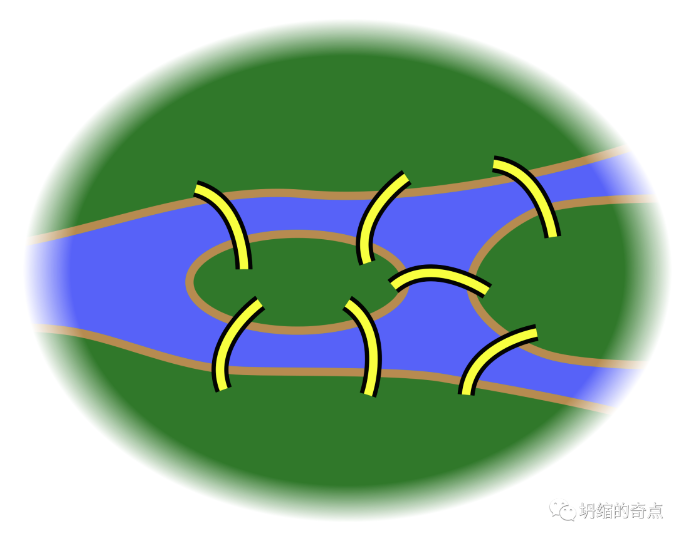
\includegraphics[width=0.5\textwidth]{asset/20231227144751.png}
  \caption{}
  \label{fig:img24_1}
\end{figure}

格里斯堡问题用数学化的模型可以给它抽象成点线的模型, 点就代表了河的两岸, 以及河中间的小岛. 线就代表着桥, 所以问题就可以抽象成能不能从任意一点出发, 不重不漏的走过每一个桥, 最终回到起点. (图:\ref{fig:img24_2})

\begin{figure}[ht]
  \centering
  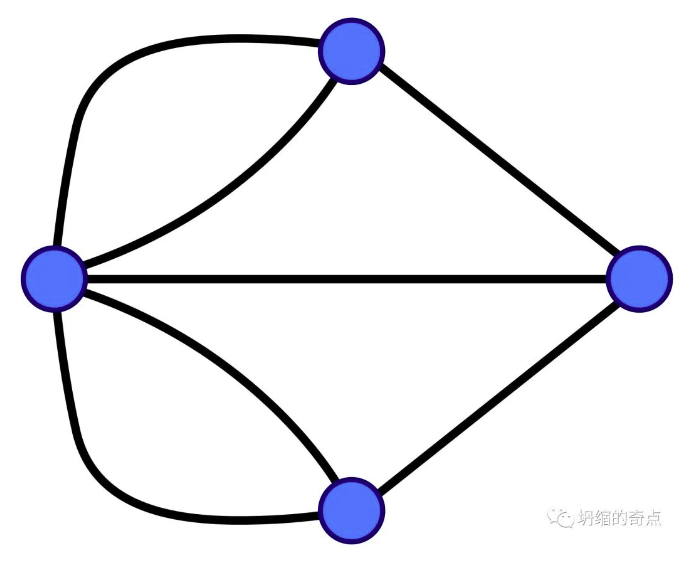
\includegraphics[width=0.4\textwidth]{asset/20231227144732.png}
  \caption{}
  \label{fig:img24_2}
\end{figure}

很多人花了很长时间去研究这个问题, 但最终也没找到一个解. 后来这个问题被证明, 是找不到这样一种解法的, 或者说找不到这样的路线可以满足这样的条件. 由此, 也催生出了图论这门科学的一个产生. 

然后, 图除了一开始是由这种对现实世界的格里斯堡问题抽象得来的之外, 在当代世界我们还有哪一些地方可以用得到这个图呢?

在化学研究当中也是需要用到图的, 很多同学学过高中化学的应该会有印象. 我们描述一个物体的结构, 尤其是有机物的时候, 一般是用结构式或者结构简式去表示. 这种结构的表示方法其实就用到了图的形式. 

比如, 丁烷($c_4H_10$)不管是正丁烷还是异丁烷, 它都是点线模型. 和我们刚才说的格力斯堡问题很像(图: \ref{fig:img24_3}). 

\begin{figure}[ht]
  \centering
  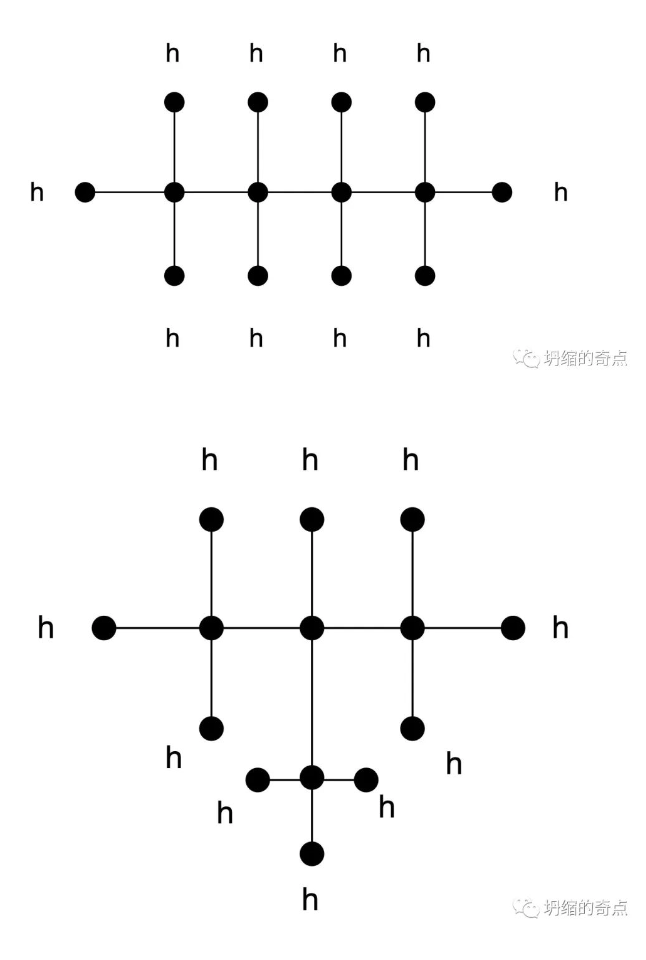
\includegraphics[width=0.5\textwidth]{asset/20231227144811.png}
  \caption{}
  \label{fig:img24_3}
\end{figure}

同样的, 除了这些科学领域之外, 我们的社会生活, 日常生活里面也是大量用到图的. 比如说高铁的运营线路, 各大城市的地铁网络, 这些其实都是用图这种结构去给它做的一个抽象. 为什么说是抽象呢, 因为在这个高铁线路图上面你看到这两个点, 或者这条线上面这些距离不一定代表它真实的距离(图: \ref{fig:img24_4}). 

\begin{figure}[ht]
  \centering
  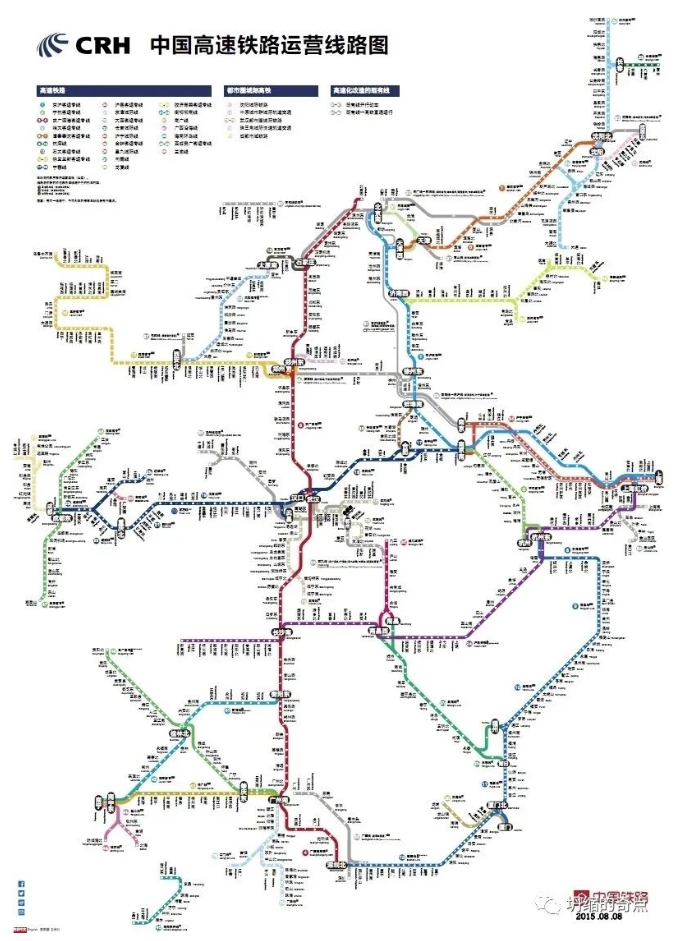
\includegraphics[width=0.5\textwidth]{asset/20231227144832.png}
  \caption{}
  \label{fig:img24_4}
\end{figure}

看似这条线段会比较长, 但是在实际当中也许不一定会长. 它只是表示了这个线路会经过哪些点, 以及在哪些点的位置会和其他线交汇, 更多的是一种定性的表示, 而不是一种定量的表示. 

同样的, 还有一个应用也非常有趣, 我以前就很好奇这个期末考试的时间. 比如一个大学里面那么多的专业, 每一个专业里面还分那么多班, 那这些考试要怎么样去安排呢?因为考试和这个平时上课不一样, 平时上课的时候大家可以挤在一个阶梯教室里面, 紧挨着. 也不用顾虑中间有没有人, 或者别人能不能看到你, 正在看的这些东西啊什么的. 但是考试不一样, 考试必须得中间隔一个位置. 这样的话代表了平时正好足够装满那么多学生的教室到了考试的时候就不够用了. 所以这些考试不管是同专业也好, 不同专业也好, 都得需要去进行一个排布. 

排布的话问题就来了, 怎么样避免时间上的一个冲突呢?这里其实同样可以用图的知识来解答. 是不是很有趣?怎么样解答呢?

首先我们把它抽象成图的模型, 如图\ref{fig:img24_5}, 因为我们知道图是由顶点和边来组成的, 顶点代表了这些待排布的课程考试. 连接两个顶点的边表示有学生是同时选择这两门课程的, 所以被同一条边连接的两个顶点能不能放在同一个时间段去安排考试?不行的对吧. 

\begin{figure}[ht]
  \centering
  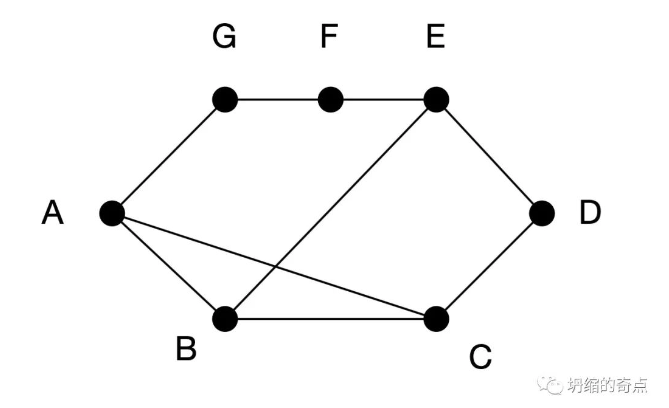
\includegraphics[width=0.5\textwidth]{asset/20231227144844.png}
  \caption{}
  \label{fig:img24_5}
\end{figure}

所以这个问题又可以进一步的转化为用不同的颜色去给这些顶点上色, 然后要求不同时间段的考试, 这里的顶点需要用不同的颜色, 相同时间段的考试用相同的颜色. 

也就是说我们一条边所连接的两个顶点不能是同色的. 同色代表了考试的时间被安排在同一个时间段, 而他被一条边连接, 说明有学生同时选择这两门课. 同学又没有分身术, 这样就会产生一个很严重的问题. 所以呢, 我们通过一个图的一个转化, 就把这种时间安排的问题给他转成了一个上色问题. 可能有的同学知道这一点, 就是四色问题. 就是说怎么样用四种颜色给世界地图去上色. 每个国家都用一种颜色, 然后相互接壤的国家不能用同一种颜色, 问 4 个颜色够不够. 

这个就是一个例子, 比如说有 ABCDEFG 这 7 门考试, 然后你看 BE 它是被连接在一起的, 所以 B 点和 E 点肯定不能上同样的颜色. 同样的 AC, 以及任意相邻的这两点都是一样的. 那 A、D 就可以用同样的颜色. 

\section{图的构成}

我们在讨论课里面其实也有给大家介绍过图是怎么样的一个东西. 

首先, 我们直观的来理解的话是由顶点和边构成的, 这个我们已经很清楚了. 虽然导论课里面我们说的很不深入, 但是基本的概念我们都有所了解. 顶点和边共同在一起就组成了这些图 \ref{fig:img24_6}. 

\begin{figure}[ht]
  \centering
  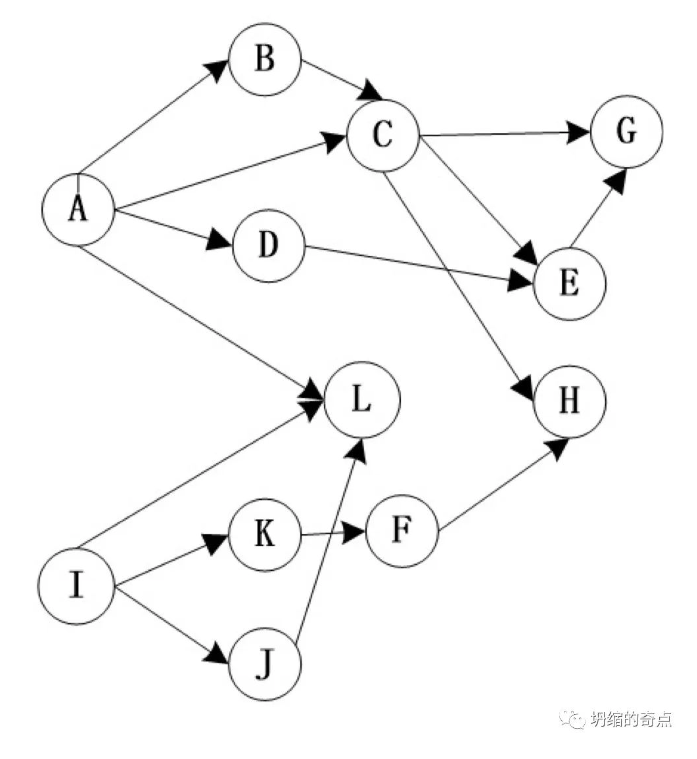
\includegraphics[width=0.5\textwidth]{asset/20231227144901.png}
  \caption{}
  \label{fig:img24_6}
\end{figure}

那还有一个问题, 就是图呢, 我们知道了它由点和线来表示之后, 我们需要关心的是哪些点?我们不需要关心的是哪些点呢?

首先, 我们需要关心这个图里面有多少个顶点. 以及这些顶点之间是否有这些边, 或者说这些线来连接. 我们不关心的东西是这个边具体是多长 \ref{fig:img24_7}. 

\begin{figure}[ht]
  \centering
  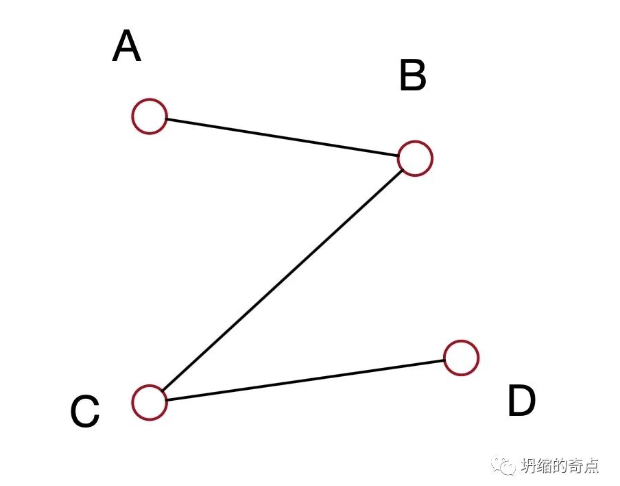
\includegraphics[width=0.3\textwidth]{asset/20231227144917.png}
  \caption{}
  \label{fig:img24_7}
\end{figure}

比如 BC 的连线比 AB 的连线要长, 那它是否代表了特殊的含义呢?或者说所有的连线画成的都是直线的形状, 那是否代表着直线和弯线代表着不同含义呢?以及 C 是在 A 的正下方, 在 D 的正左方. 这样子的话它们是不是表示一种位置上的含义呢?

答案都是否定的. 

这些图是一种高度抽象的模型, 刚才也说了, 它往往是一种定性的分析, 而不是一种定量的. 大家可以想象一下那个高铁线路图, 不是说在这个高铁线路图上面看着比较长的线段就真的在现实生活中比其他的高铁线路要长, 只是一种相对的位置关系. 所以我在这里列出的这三点呢都不是我们考虑的范围. 

比如我把 A、B 连线弄成一段圆弧, 弄成一个劣弧优弧都可以, 或者把它给那个弄成一个波浪形, 其实和直线一样, 完全没有任何影响. 

接下来, 我们要接触比较让人脑壳疼的数学部分. 如果我们给图一个正式的定义, 它会是怎么样子呢?

首先我们来看一下, 一个图是一个序偶$<V,E>$, 符号表示为$G = <V, E>$. 

这个 V 和 E 符号表示什么?G 就代表了图, 英语 Graft 首字母, 我们用它来代表图. \(V = {V1, V2, V3, ..., Vn}\), 是一个有限非空集合, Vi 称为顶点, 或者简称为点. V 代表了这些顶点的集合, 称为顶点集,  用\(|V|\)表示顶点数. 

这是一种比较常用的一种表示方法. 这个不光是表示图, 在集合里面往往我们也用这种表示方法, 就用绝对值的符号扩起来这个集合的字母, 就代表了这个集合的元素数量. 

E 也是一个有限集合, 是一个图的所有边的集合, 称为边集. 它和 V 是相对的, 一个是囊括了所有的顶点, 一个是囊括了所有的边. E 是英文 edge 的首字母, 表示边. E 中的每个元素都有 v 中的节点对与之对应, 用|E|表示变数. 

边肯定是有两个端点的, 这两个端点就对应着这个图的顶点. 这也是很容易想象的, 所以它说是和 V 中的顶节点对应. 

这里有一点大家需要注意一下, 就是在这里呢我们说到 V, 它是一个有限非空集合. 在 E 这里, 我们并没有说它一定要求是非空的, 这一点大家稍微注意一下. 

关于图, 有一些常见图的名词解释, 这些名词解释本身的意义都非常的简单. 如果你知道顶点和边是啥之后, 这些名词理解它不会有什么问题. 唯一的问题可能出在哪呢, 就是之后可能记不住这么多名词. 但是没关系, 我们的一个宗旨是你到用的时候再回来查. 慢慢的, 一次、两次、三次, 次数多了之后, 就算是一个记性特别差的人都能记得住. 

\begin{itemize}
  \item 有限图: 顶点数和边数都有限的图. 
  \item 空图: 边集为空(无边)的图. 边集为空, 就是说它没有边. 这个也说明什么, 我们之前说到, E 并没有要求是非空的. 就说明了一个图它必须有顶点, 但是可以没有边. 这种就被称为空图. 要记住, 空图不是说它里面啥都没有, 只是没有边而已. 
  \item 平凡图: 只有一个顶点的图. 
  \item n 阶图: 顶点数为 n 的图. 所以, 我们其实就是把顶点数为几的图就叫做几阶图. 
  \item $(n,m)$图: 顶点数为 n, 边数为 m 的图. 这个就跟直角坐标那个点的坐标一样. 一个 n、一个 m 分别对应着顶点数和边数. 
  \item 环: 端点重合为一点的边. 比如图\ref{fig:img24_8}, 
\end{itemize}

\begin{figure}[ht]
  \centering
  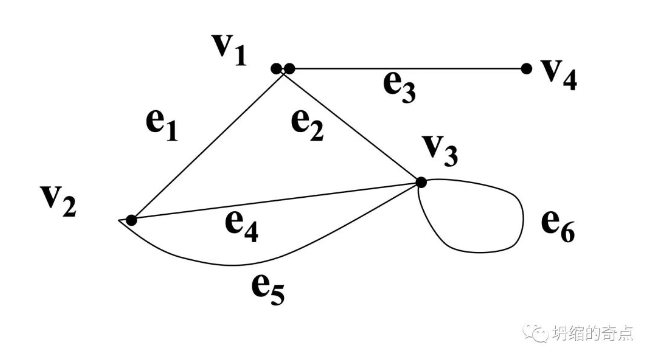
\includegraphics[width=0.5\textwidth]{asset/20231227144939.png}
  \caption{}
  \label{fig:img24_8}
\end{figure}

图\ref{fig:img24_8}里面$e6$就是顶点相互重合的. 它不像其他的边是由两个端点构成的, $e6$在这里两个端点重合为 V3,所以它就是一个环. 

\begin{itemize}
  \item 重边: 链接两个相同顶点的多条边(大于 1 条), 边的条数称作为边的重数. 还是上图, V2 和 V3 之间是不是不光有一条边, 它有两条, e4 和 e5. 边的条数就称为这个边的重数. 
  \item 简单图: 图中没有环且没有重边. 就是这个图里面非常纯粹, 它没有环也没有重边, 干干净净的, 不会让你产生其他的困扰, 没有比较特殊的结构. 因为环起点终点都是一样的, 所以它有些特殊的性质. 重边对应着路径不唯一, 所以也带来一定的复杂性. 所以, 如果没有这两个折磨人的小妖精的话, 那我们就把这个图称为简单图. 
  \item 复合图: 图中有环或者有重边, 或者两者均有. 就带来一些复杂性. 
\end{itemize}

好, 我们说到这里, 需要大家掌握到什么程度呢?你在看我讲解的时候, 你理解这些东西是什么意思就 OK 了. 至于是否能一下子全部记住这些内容一点都不重要, 只要能理解就 OK. 

那这个也是我们关于图论的第一节课说要讲述的内容, 先让大家熟悉一下相关概念和名词. 因为对于之前我们说讲的内容, 包括微积分、线性代数和概率统计, 大部份人起码是接触过有一定概念的, 但是图论应该很多人都没有接触过. z